\documentclass{ajc}
\usepackage[output-decimal-marker={,},per-mode=fraction,fraction-function=\tfrac]{siunitx}
\mathcode`,="002C
\numberwithin{equation}{subsection}
\newcommand\numberthis{\addtocounter{equation}{1}\tag{\theequation}}


\title{Mathe}
\author{Alexander Jacob}
\date{Schuljahr 2024/2025}

\begin{document}
	\section{Vektoren}
	\subsection{Spurpunkte berechnen}
	\paragraph{a)} Bestimmen Sie die Spurpunkte der Geraden
	\begin{equation}
		\mathbf{g}: \overrightarrow{x}=\left(\begin{array}{r} 2 \\ 1 \\ 7\end{array}\right) + \lambda \cdot \left(\begin{array}{r} 0 \\ 6 \\ 4\end{array}\right) \text{\quad und \quad} \mathbf{h}: \overrightarrow{x}=\left(\begin{array}{r} -3 \\ 0 \\ -5\end{array}\right) + \mu \cdot \left(\begin{array}{r} 1 \\ 3 \\ 2\end{array}\right). 
	\end{equation}
	
	\subparagraph{zu g:}
	\begin{equation}
		\overrightarrow{x}=\left(\begin{array}{r} 2 \\ 1 + 6\lambda \\ 7 + 4\lambda \end{array}\right)
	\end{equation}
	
	Bedingung für Spurpunkt mit $x_1\text{-}x_2$-Ebene:\quad $x_3 = 0$
	
	Punkt von \textbf{g} in der $x_1\text{-}x_2$-Ebene:\quad $x_3 = 0 \Leftrightarrow 0 = 7 + 4\lambda \Leftrightarrow \lambda = -\frac{7}{4}$
	
	Ortsvektor des Spurpunkts: 
	\begin{equation}
	\overrightarrow{s_\text{12}}=\left(\begin{array}{r} 2 \\ -9,5 \\ 0\end{array}\right)
	\end{equation}
	Spurpunkt: $S_\text{12}(2|-9,5|0)$
	
	Bedingung für Spurpunkt mit $x_1\text{-}x_3$-Ebene:\quad $x_2 = 0$
	
	Punkt von \textbf{g} in der $x_1\text{-}x_3$-Ebene:\quad $x_2 = 0 \Leftrightarrow 0 = 1 + 6\lambda \Leftrightarrow \lambda = -\frac{1}{6}$
	
	Ortsvektor des Spurpunkts: 
	\begin{equation}
		\overrightarrow{s_\text{13}}=\left(\begin{array}{r} 2 \\ 0 \\ 6,\overline{3}\end{array}\right)
	\end{equation}
	Spurpunkt: $S_\text{12}(2|0|6,\overline{3})$
	
	Bedingung für Spurpunkt mit $x_2$-$x_3$-Ebene:\quad $x_1 = 0$
	
	Punkt von \textbf{g} in der $x_2\text{-}x_3$-Ebene:\quad $x_1 = 0 \Leftrightarrow 0 \ne 2 \,\lightning$
	
	Es gibt keinen Spurpunkt von $g$ in der $x_2\text{-}x_3$-Ebene.
	
	\subparagraph{zu h:}
	\begin{equation}
		\overrightarrow{x}=\left(\begin{array}{r} -3 + \mu \\ 3\mu \\ -5 + 2\mu\end{array}\right)
	\end{equation}
	
	Bedingung für Spurpunkt mit $x_1\text{-}x_2$-Ebene:\quad $x_3 = 0$
	
	Punkt von \textbf{h} in der $x_1\text{-}x_2$-Ebene:\quad $x_3 = 0 \Leftrightarrow 0 = -5 + 2\mu \Leftrightarrow \mu = \frac{5}{2}$
	
	Ortsvektor des Spurpunkts: 
	\begin{equation}
		\overrightarrow{s_\text{12}}=\left(\begin{array}{r} -0,5 \\ 7,5 \\ 0\end{array}\right)
	\end{equation}
	Spurpunkt: $S_\text{12}(-0,5|7,5|0)$
	
	Bedingung für Spurpunkt mit $x_1\text{-}x_3$-Ebene:\quad $x_2 = 0$
	
	Punkt von \textbf{h} in der $x_1\text{-}x_3$-Ebene:\quad $x_2 = 0 \Leftrightarrow 0 = 3\mu \Leftrightarrow \mu = 0$
	
	Ortsvektor des Spurpunkts: 
	\begin{equation}
		\overrightarrow{s_\text{13}}=\left(\begin{array}{r} -3 \\ 0 \\ -5\end{array}\right)
	\end{equation}
	Spurpunkt: $S_\text{12}(-3|0|-5)$
	
	Bedingung für Spurpunkt mit $x_2$-$x_3$-Ebene:\quad $x_1 = 0$
	
	Punkt von \textbf{h} in der $x_2\text{-}x_3$-Ebene:\quad $x_1 = 0 \Leftrightarrow 0 = -3 + \mu \Leftrightarrow \mu = 3$
	
	Ortsvektor des Spurpunkts: 
	\begin{equation}
		\overrightarrow{s_\text{23}}=\left(\begin{array}{r} 0 \\ 9 \\ 1\end{array}\right)
	\end{equation}
	Spurpunkt: $S_\text{23}(0|9|1)$
	
	
	\paragraph{b)} Von einer Geraden sind die Spurpunkte $S_\text{12} (2|3|0)$ und \linebreak $S_\text{23} (0|-1|1)$ bekannt. Bestimmen Sie den Spurpunkt $S_\text{13}$.
	
	Zweipunktegleichung einer Geraden:
	\begin{equation}\label{eq:1.1zpg}
		\mathbf{g}: \overrightarrow{x}= \vec{a} + \lambda \cdot \left(\overrightarrow{b} - \overrightarrow{a}\right)
	\end{equation}
	
	Mit den eingesetzten Punkten $S_\text{12}$ und $S_\text{23}$ in \ref{eq:1.1zpg} ergibt sich:
	\begin{equation}\label{eq:1.1zpg_ein}
		\mathbf{g}: \overrightarrow{x}= \left(\begin{array}{r} 2 \\ 3 \\ 0\end{array}\right) + \lambda \cdot \left(\begin{array}{r} -2 \\ -4 \\ 1\end{array}\right) = \left(\begin{array}{r} 2 - 2\lambda \\ 3 - 4\lambda \\ \lambda\end{array}\right)
	\end{equation}
	
	Bedingung für Spurpunkt mit $x_1\text{-}x_3$-Ebene:\quad $x_2 = 0$
	
	Punkt von \textbf{g} in der $x_1\text{-}x_3$-Ebene:\quad $x_2 = 0 \Leftrightarrow 0 = 3 - 4\lambda \Leftrightarrow \lambda = \frac{3}{4}$
	
	Ortsvektor des Spurpunkts: 
	\begin{equation}
		\overrightarrow{s_\text{13}}=\left(\begin{array}{r} 0,5 \\ 0 \\ 0,75\end{array}\right)
	\end{equation}
	Spurpunkt: $S_\text{12}(0,5|0|0,75)$
	
	\subsection{Pyramide}
	Gegeben ist eine gerade Pyramide mit quadratischer Grundfläche. Die Seitenlänge des in der $x_1$-$x_2$-Ebene liegenden Quadrates ABCD beträgt 80 m, die Pyramide hat eine Höhe von 60 m.
	
	Die Richtung der einfallenden Sonnenstrahlen ist gegeben durch den Vektor $\overrightarrow{u}=\left(\begin{array}{r} 2 \\ 4 \\ -3\end{array}\right)$.
	
	Der Schattenpunkt $S'$ der Pyramidenspitze $S$ liegt in der $x_1$-$x_2$-Ebene.
	Berechnen Sie die Koordinaten von $S'$.
	
	\begin{figure}[ht]
		\centering
		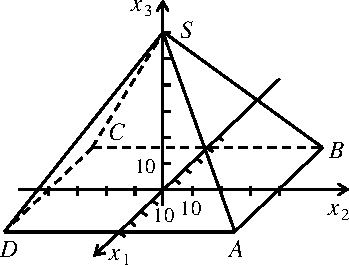
\includegraphics[width=0.5\textwidth]{ma_002_pyramide.pdf}
		\caption{Skizze der Pyramide.}
		\label{fig:002_pyramide}
	\end{figure}

	Vektor der auf Punkt $S$ fallenden Sonnenstrahlen:
	\begin{equation}
		\overrightarrow{x}=\left(\begin{array}{r} 0 \\ 0 \\ 60\end{array}\right) + \lambda \cdot \left(\begin{array}{r} 2 \\ 4 \\ -3\end{array}\right)
	\end{equation}
	
	Bedingung für Spurpunkt mit $x_1$-$x_2$-Ebene:\quad $x_3 = 0$

	Punkt in der $x_1$-$x_2$-Ebene: $0 = 60 -3 \lambda \Leftrightarrow 60 = 3\lambda \Leftrightarrow \lambda = 20$
	
	Schattenpunkt: $S'(40|80|0)$
	
	\subsection{Schatten einer Plakatwand}
	Vor einem Haus steht eine Plakatwand, die \SI{3}{\m} breit und \SI{6}{m} hoch ist. Ein Punkt der Wand ist $A(6|2|6)$. Auf die Plakatwand fällt paralleles Sonnenlicht. Die Richtung der Sonnenstrahlen ist gegeben durch den Vektor
	\begin{equation*}
		\overrightarrow{u}=\left(\begin{array}{r} -3 \\ 1 \\ -1\end{array}\right).
	\end{equation*}
	Bestimmen und beschreiben Sie den Verlauf des Schattens an der Hauswand und auf dem Boden.
	
	\begin{figure}[ht]
		\centering
		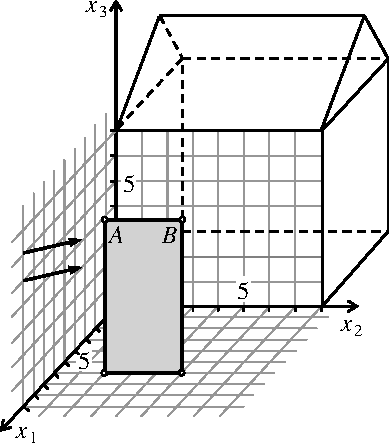
\includegraphics[width=0.5\textwidth]{ma_001_schatten.pdf}
		\caption{Skizze der Plakatwand mit Hauswand.}
		\label{fig:001_schatten}
	\end{figure}
	
	Geraden in Richtung des Sonneneinfalls:
	\begin{equation}
		\mathbf{g}: \overrightarrow{x}=\left(\begin{array}{r} 6 \\ 2 \\ 6\end{array}\right) + \lambda \cdot \left(\begin{array}{r} -3 \\ 1 \\ -1\end{array}\right) = \left(\begin{array}{r} 6 - 3 \lambda \\ 2 + \lambda \\ 6 - \lambda\end{array}\right)
	\end{equation}
	\begin{equation}
		\mathbf{h}: \overrightarrow{x}=\left(\begin{array}{r} 6 \\ 5 \\ 6\end{array}\right) + \mu \cdot \left(\begin{array}{r} -3 \\ 1 \\ -1\end{array}\right) = \left(\begin{array}{r} 6 - 3 \mu \\ 5 + \mu \\ 6 - \mu\end{array}\right)
	\end{equation}
	
	Gesucht sind jeweils die Spurpunkte von \textbf{g} und \textbf{h} mit der $x_2\text{-}x_3$-Ebene (= Hauswand).
	
	Bedingung für Spurpunkt mit $x_2$-$x_3$-Ebene:\quad $x_1 = 0$
	
	\paragraph{Für g gilt:} 
	
	Punkt von \textbf{g} in der $x_2\text{-}x_3$-Ebene:\quad $x_1 = 0 \Leftrightarrow 0 = 6 - 3 \lambda \Leftrightarrow \lambda = 2$
	
	Ortsvektor des Spurpunkts: 
	\begin{equation}
		\overrightarrow{s_\text{A23}}=\left(\begin{array}{r} 0 \\ 4 \\ 4\end{array}\right)
	\end{equation}
	Spurpunkt: $S_\text{23}(0|4|4)$
	
	\paragraph{Für h gilt:} 
	
	Punkt von \textbf{h} in der $x_2\text{-}x_3$-Ebene:\quad $x_1 = 0 \Leftrightarrow 0 = 6 + -3 \mu \Leftrightarrow \mu = 2$
	
	Ortsvektor des Spurpunkts: 
	\begin{equation}
		\overrightarrow{s_\text{B23}}=\left(\begin{array}{r} 0 \\ 7 \\ 4\end{array}\right)
	\end{equation}
	Spurpunkt: $S_\text{B23}(0|7|4)$
	
	Der Schatten der Plakatwand fällt also zum Teil auf die Hauswand bis auf eine Höhe von \SI{4}{\meter} mit einer Breite von \SI{3}{\meter}. Der andere Teil des Schattens fällt demnach auf den Boden vor der Hauswand zwischen den Punkten $A_0$, $B_0$, $S_{A0}$ und $S_{B0}$. Für diese Punkte gilt, dass sie senkrecht unter den Punkten $A$, $B$, $S_\text{A23}$ und $S_\text{B23}$ auf der $x_1\text{-}x_2$-Ebene liegen. Es gilt: $A_0 = (6|2|0)$, $B_0 = (6|5|0)$, $S_{A0} = (0|4|0)$ und $S_{B0} = (0|7|0)$.
	
	\subsection{Lageuntersuchung von Geraden}
	Untersuchen Sie die Geraden \textbf{g} und \textbf{h} auf ihre gegenseitige Lage. Berechnen Sie gegebenenfalls den Schnittpunkt.
	
	\begin{equation}
		\mathbf{g}: \overrightarrow{x}=\left(\begin{array}{r} -11 \\ 9 \\ 1\end{array}\right) + \lambda \cdot \left(\begin{array}{r} -4 \\ 3 \\ -2\end{array}\right) \text{\quad ; \quad} \mathbf{h}: \overrightarrow{x}=\left(\begin{array}{r} -4 \\ 11 \\ 4\end{array}\right) + \mu \cdot \left(\begin{array}{r} 3 \\ 5 \\ 1\end{array}\right)
	\end{equation}
	
	\begin{itemize}
		\item \textit{Test auf Parallelität} \\ 
		Die Richtungsvektoren sind nicht kollinear, daher sind die Geraden nicht parallel.
		
		\item \textit{Lageentscheidung (Gleichsetzungsverfahren)} \\
		\begin{alignat*}{2}
			\left(\begin{array}{r} -11 \\ 9 \\ 1\end{array}\right) + \lambda \cdot \left(\begin{array}{r} -4 \\ 3 \\ -2\end{array}\right) &= \left(\begin{array}{r} -4 \\ 11 \\ 4\end{array}\right) + \mu \cdot \left(\begin{array}{r} 3 \\ 5 \\ 1\end{array}\right) \\
			&\iff \left(\begin{aligned} -4 \lambda - 3 \mu &= 7 \\ 3 \lambda - 5 \mu &= 2 \\ -2 \lambda  - 1 \mu &= 3 \end{aligned}\right) \begin{array}{c} \text{(I)} \\ \text{(II)} \\ \text{(III)}\end{array} \numberthis
		\end{alignat*}
		
		Lösung: $\begin{array}{l}
			3\cdot\text{(III)} - \text{(I)}: \quad -2\lambda = 2 \Leftrightarrow \lambda = -1 \\ \text{Einsetzen in (III)}: \quad 2 - \mu = 3 \Leftrightarrow \mu = -1 \\ \text{Probe in  (I)}: \quad -4\cdot(-1) -3\cdot(-1) = 7 \checkmark \end{array}$
			
		Das Gleichungssystem ist für $\lambda = -1$ und $\mu = -1$ erfüllt, somit gibt es einen Schnittpunkt. \\
		\item \textit{Schnittpunktberechnung} \\
		$\lambda$ in $g$ eingesetzt gibt: 
		\begin{equation}
			\overrightarrow{x}=\left(\begin{array}{r} -11 \\ 9 \\ 1\end{array}\right) -1 \cdot \left(\begin{array}{r} -4 \\ 3 \\ -2\end{array}\right) = \left(\begin{array}{r} -7 \\ 6 \\ 3\end{array}\right)
		\end{equation}
		Die Geraden scheiden sich im Punkt $S(-7|6|3)$.
	\end{itemize}
	
	\subsection{Flugzeugcrash}
	Ein Passagierflugzeug $\text{F}_1$ befindet sich im Punkt  $A(10|30|2)$ und fliegt geradlinig in Richtung des Punktes $B(40|90|2)$. Ein Sportflugzeug $\text{F}_2$ befindet sich zum gleichen Zeitpunkt im Punkt $C(70|90|11)$ und nimmt Kurs auf den Punkt $D(70|110|8)$ (alle Angaben in km).
	
	\begin{figure}[ht]
		\centering
		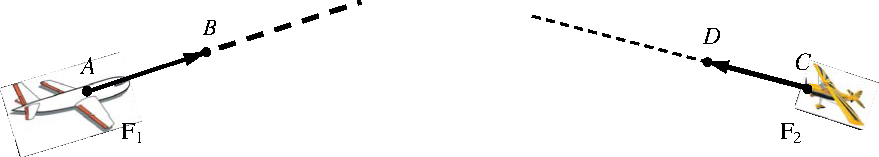
\includegraphics[width=\textwidth]{ma_003_flugzeuge.pdf}
		\caption{Skizze der Flugzeuge.}
		\label{fig:003_flugzeuge}
	\end{figure}
	
	\paragraph{a)} Begründen Sie, dass sich die beiden Flugzeuge auf Kollisionskurs befinden.
	
	\subparagraph{zu $\text{F}_1$:} Mit den eingesetzten Punkten $A$ und $B$ in die Zweipunktegleichung \ref{eq:1.1zpg} ergibt sich: 
	\begin{equation}
		\mathbf{F_1}: \overrightarrow{x}=\left(\begin{array}{r} 10 \\ 30 \\ 2\end{array}\right) + \lambda \cdot \left(\begin{array}{r} 30 \\ 60 \\ 0\end{array}\right)
	\end{equation}
	
	\subparagraph{zu $\text{F}_2$:} Mit den eingesetzten Punkten $C$ und $D$ in die Zweipunktegleichung \ref{eq:1.1zpg} ergibt sich: 
	\begin{equation}
		\mathbf{F_2}: \overrightarrow{x}=\left(\begin{array}{r} 70 \\ 90 \\ 11\end{array}\right) + \mu \cdot \left(\begin{array}{r} 0 \\ 20 \\ -3\end{array}\right)
	\end{equation}
	
	\begin{itemize}
		\item \textit{Test auf Parallelität} \\ 
		Die Richtungsvektoren sind nicht kollinear, daher sind die Geraden nicht parallel.
		
		\item \textit{Lageentscheidung (Gleichsetzungsverfahren)} \\
		\begin{alignat*}{2}
			\left(\begin{array}{r} 10 \\ 30 \\ 2\end{array}\right) + \lambda \cdot \left(\begin{array}{r} 30 \\ 60 \\ 0\end{array}\right) &= \left(\begin{array}{r} 70 \\ 90 \\ 11\end{array}\right) + \mu \cdot \left(\begin{array}{r} 0 \\ 20 \\ -3\end{array}\right) \\
			&\iff \left(\begin{aligned} 30 \lambda &= 60 \\ 60 \lambda - 20 \mu &= 60 \\ -3 \mu &= 9 \end{aligned}\right) \begin{array}{c} \text{(I)} \\ \text{(II)} \\ \text{(III)}\end{array} \numberthis
		\end{alignat*}
		
		Lösung: $\begin{array}{l}
			\text{(I) nach } \lambda: \quad 30 \lambda = 60 \Leftrightarrow \lambda = 2 \\ \text{(III) nach } \mu: \quad 3\mu = 9 \Leftrightarrow \mu = 3 \\ \text{Probe in  (II)}: \quad 60\cdot2 -20\cdot3 = 60 \checkmark \end{array}$
		
		Das Gleichungssystem ist für $\lambda = 2$ und $\mu = 3$ erfüllt, somit gibt es einen Schnittpunkt.
		
		\item \textit{Schnittpunktberechnung} \\
		$\lambda$ in $\text{F}_1$ eingesetzt gibt: 
		\begin{equation}
			\overrightarrow{x}=\left(\begin{array}{r} 10 \\ 30 \\ 2\end{array}\right) + 2 \cdot \left(\begin{array}{r} 30 \\ 60 \\ 0\end{array}\right) = \left(\begin{array}{r} 70 \\ 150 \\ 2\end{array}\right)
		\end{equation}
		Die Flugzeuge fliegen beide durch den Punkt $S(70|150|2)$.
	\end{itemize}
	
	\paragraph{b)} Prüfen Sie, ob es tatsächlich zum Crash kommt, wenn sich $\text{F}_1$ mit der Geschwindigkeit 800 km/h, $\text{F}_2$ mit 350 km/h bewegt.
	
	Verbindungsvektor zwischen $A$ und $S$:
	\begin{equation}
		\overrightarrow{f_1} = \left(\begin{array}{r} 70 - 10 \\ 150 - 30 \\ 2 - 2\end{array}\right) = \left(\begin{array}{r} 60 \\ 120 \\ 0\end{array}\right) 
	\end{equation}
		
	Länge des Verbindungsvektors zwischen $A$ und $S$:
	\begin{equation}
		\left|\overrightarrow{f_1}\right| = \sqrt{60^2 + 120^2 + 0^2} \approx \SI{134,16}{km}
	\end{equation}
	
	Zeit bis zum Eintreffen:
	\begin{equation}
		\frac{\SI{134,16}{km}}{\SI{800}{\km\per\hour}} \approx \SI{0,1677}{\hour}
	\end{equation}
	
	Verbindungsvektor zwischen $C$ und $S$:
	\begin{equation}
		\overrightarrow{f_2} = \left(\begin{array}{r} 70 - 70 \\ 150 - 90 \\ 2 - 11\end{array}\right) = \left(\begin{array}{r} 0 \\ 60 \\ -9\end{array}\right) 
	\end{equation}
	
	Länge des Verbindungsvektors zwischen $C$ und $S$:
	\begin{equation}
		\left|\overrightarrow{f_2}\right| = \sqrt{0^2 + 60^2 + (-9)^2} \approx \SI{60,67}{km}
	\end{equation}
	
	Zeit bis zum Eintreffen:
	\begin{equation}
		t_2 = \frac{\SI{60,67}{km}}{\SI{350}{\km\per\hour}} \approx \SI{0,1733}{\hour}
	\end{equation}
	
	Es kommt vermutlich zum Crash, weil beide Flugzeuge zu einem sehr ähnlichen Zeitpunkt im Punkt $S$ eintreffen werden.
	
	\subsection{Rathaus (Abituraufgabe)}
	Ein Rathaus besteht aus einem Quader mit aufgesetztem Walmdach (siehe \ref{fig:004_rathaus}; Maße in Meter).
	
	\begin{figure}[ht]
		\centering
		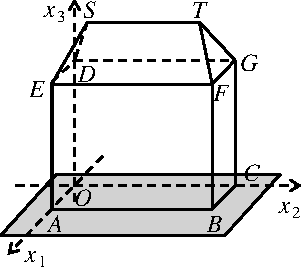
\includegraphics[width=.5\textwidth]{ma_004_rathaus.pdf}
		\caption{Skizze des Rathauses.}
		\label{fig:004_rathaus}
	\end{figure}
	
	Gegeben sind die Punkte $D(0|0|15)$, $E(8|0|15)$, $F(8|20|15)$, \linebreak $G(0|20|15)$ und $T(4|17|21)$.
	
	Neben dem Rathaus steht im Punkt $F_1(4|37|0)$ ein \SI{13}{\m} hoher senkrechter Fahnenmast mit der Spitze $F_2$.
	
	Der Vektor $\overrightarrow{v}=\left(\begin{array}{r} 1 \\ -17 \\ -11\end{array}\right)$ gibt die Richtung des einfallenden Sonnenlichts an.
	
	\paragraph{a)} Zeigen Sie, dass der Schatten des Mastes $\overline{F_1F_2}$ eine Rathauswand trifft.
	
	Geradengleichung Schattenspitze:
	\begin{equation}
		\mathbf{g}: \overrightarrow{x}=\left(\begin{array}{r} 4 \\ 37 \\ 13\end{array}\right) + \lambda \cdot \left(\begin{array}{r} 1 \\ -17 \\ -11\end{array}\right) = \left(\begin{array}{r} 4 + \lambda \\ 37 - 17 \lambda \\ 13 - 11 \lambda\end{array}\right)
	\end{equation}
	
	Da der Fahnenmast in positiver $x_2$-Richtung zum Rathaus steht, kann der Schatten nur auf die Wand $BCGF$ fallen.
	
	Bedingung für Spurpunkt auf Wand (= Ebene): $x_2 = 20$
	
	Punkt in Wand von $\mathbf{g}$: $x_2 = 20 = 37 - 17 \lambda \Leftrightarrow \lambda = 1$ 
	
	Einsetzen von $\lambda$ in $\mathbf{g}$:
	\begin{equation}
		\vec{f_2'} = \left(\begin{array}{r} 5 \\ 20 \\ 2 \end{array}\right)
	\end{equation}
	
	Die Spitze des Rathausmastes liegt also in $F_2'(5|20|2)$ und damit auf der Rathauswand.
	
	\paragraph{b)} Berechnen Sie die gesamte Länge des Schattens.
	
	An der Kante zwischen Haus und Boden macht der Schatten senkrecht unter seiner Spitze einen Knick im Punkt $K(5|20|0)$. Für die Länge dieses Schattenabschnitts gilt intuitiv: $\overline{F_2'K} = \SI{2}{\m}$.
	
	Die Strecke des Schattenabschnitts $\overline{F_1K}$ ergibt sich wie folgt:
	\begin{equation}
		\overrightarrow{f_1k} = \left(\begin{array}{r} 4 \\ 37 \\ 0\end{array}\right) - \left(\begin{array}{r} 5 \\ 20 \\ 0\end{array}\right) = \left(\begin{array}{r} -1 \\ 17 \\ 0\end{array}\right)
	\end{equation}
	
	\begin{equation}
		\overline{F_1K} = \left|\overrightarrow{f_1k}\right| = \sqrt{(-1)^2 + 17^2 + 0^2} \approx \SI{17,0}{\m}
	\end{equation}
	
	Insgesamt ergibt sich also für den Schatten eine Länge von $\overline{F_2'K} + \overline{F_1K} = \SI{19}{m}.·$
	
	\subsection{Ebenengleichungen}
	Geben Sie eine Gleichung der Ebene durch die Punkte $A$, $B$ und $C$ an.
	
	\paragraph{a)}$A(2|-4|0)$, $B(-3|1|4)$ und $C(5|0|1)$
	\begin{equation}
		e: \vec{x} = \left(\begin{array}{r} 2 \\ -4 \\ 0\end{array}\right) + \lambda \cdot \left(\begin{array}{r} -5 \\ 5 \\ 4\end{array}\right) + \mu \cdot \left(\begin{array}{r} 3 \\ -4 \\ 1\end{array}\right)
	\end{equation}
	
	\paragraph{b)}$A(1|-2|5)$, $B(-5|4|3)$ und $C(0|0|1)$
	\begin{equation}
		e: \vec{x} = \left(\begin{array}{r} 1 \\ -2 \\ 5\end{array}\right) + \lambda \cdot \left(\begin{array}{r} -6 \\ 6 \\ -2\end{array}\right) + \mu \cdot \left(\begin{array}{r} -1 \\ 2 \\ -4\end{array}\right)
	\end{equation}
	
	\subsection{Seitenflächen eines Quaders}
	Bestimmen Sie jeweils eine Parametergleichung der Ebene, in der die Seitenflächen $ABFE$ bzw. $BCGF$ des Quaders liegen.
	\begin{figure}[ht]
		\centering
		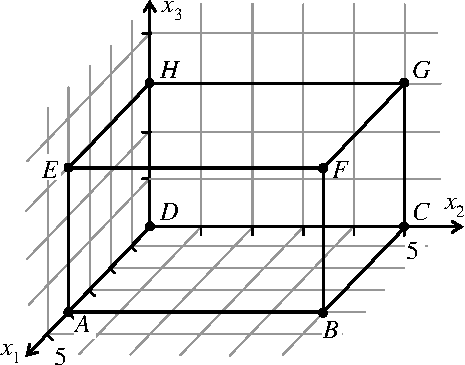
\includegraphics[width=.3\textwidth]{ma_005_quader.pdf}
		\caption{Skizze des Quaders.}
		\label{fig:005_quader}
	\end{figure}
	
	\paragraph{Seitenfläche $ABFE$:} $A(4|0|0)$, $B(4|5|0)$, $F(4|5|3)$, $E(4|0|3)$
	
	Stützvektor zum Punkt $A$ und Richtungsvektoren zu $B$ und $E$ geben:
	\begin{equation}
		e: \overrightarrow{x} = \left(\begin{array}{r} 4 \\ 0 \\ 0\end{array}\right) + \lambda \cdot \left(\begin{array}{r} 0 \\ 0 \\ 3\end{array}\right) + \mu \cdot \left(\begin{array}{r} 0 \\ 5 \\ 0\end{array}\right) \text{ mit } \lambda,\,\mu \left[0;1\right]
	\end{equation}
	
	\paragraph{Seitenfläche $BCGF$:} $B(4|5|0)$, $C(0|5|0)$, $F(0|5|3)$, $F(4|5|3)$
	
	Stützvektor zum Punkt $C$ und Richtungsvektoren zu $B$ und $G$ geben:
	\begin{equation}
		e: \overrightarrow{x} = \left(\begin{array}{r} 0 \\ 5 \\ 0\end{array}\right) + \lambda \cdot \left(\begin{array}{r} 5 \\ 0 \\ 0\end{array}\right) + \mu \cdot \left(\begin{array}{r} 0 \\ 0 \\ 3\end{array}\right) \text{ mit } \lambda,\,\mu \left[0;1\right]
	\end{equation}
	
	\subsection{Ebenen einer Pyramide}
	Gegeben ist eine Pyramide mit einem Quadrat der Seitenlänge 4 als Grundfläche sowie dem Punkt $S(2|2|4)$ als Spitze.
	\begin{figure}[ht]
		\centering
		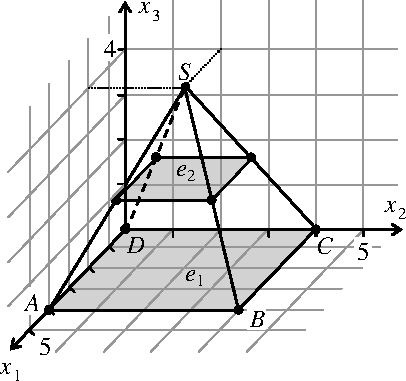
\includegraphics[width=.5\textwidth]{ma_006_pyramidepg.pdf}
		\caption{Skizze der Pyramide.}
		\label{fig:006_pyramidepg}
	\end{figure}
	
	\paragraph{a)} Bestimmen Sie eine Parametergleichung der Ebene $e_1$, in der die Bodenfläche liegt. 
	
	Entnehmen Sie die notwendigen Informationen aus der Zeichnung.
	
	Mit $D = O$ als Aufpunkt der Ebene ergibt sich für die Ebenengleichung:
	\begin{equation}
		e: \overrightarrow{x}= \lambda \cdot \left(\begin{array}{r} 1 \\ 0 \\ 0\end{array}\right) + \mu \cdot \left(\begin{array}{r} 0 \\ 1 \\ 0\end{array}\right) \text{ mit } \lambda,\,\mu \in \left[0;4\right]
	\end{equation}
	
	\paragraph{b)} Bestimmen Sie eine Parametergleichung der Ebene $e_2$, in der die Mittenfläche liegt.
	
	Für den Mittelpunkt zwischen $D$ und $S$ gilt:
	\begin{equation}
		D_m = \frac{1}{2} \left(\vec{d} + \vec{s}\right) = \left(\begin{array}{r} 1 \\ 1 \\ 2\end{array}\right)
	\end{equation}
	
	Aus der Symmetrie der Pyramide ergibt sich, dass jeder Mittelpunkt einen Abstand von $\SI{1}{LE}$ zur Spitze in $x_1$- bzw. $x_2$-Richtung besitzt. Daher gilt für die Ebenengleichung:
	\begin{equation}
		e: \overrightarrow{x}=\left(\begin{array}{r} 1 \\ 1 \\ 2\end{array}\right) + \lambda \cdot \left(\begin{array}{r} 1 \\ 0 \\ 0\end{array}\right) + \mu \cdot \left(\begin{array}{r} 0 \\ 1 \\ 0\end{array}\right) \text{ mit } \lambda,\,\mu \in \left[0;2\right]
	\end{equation}
	
	\subsection{Spiegel im Museum}
	In der Ecke eines großen Museumsraumes wurde für eine Kunstinstallation entsprechend der Abbildung \ref{fig:007_spiegel} ein dreieckiger Spiegel eingebaut. 
	\begin{figure}[ht]
		\centering
		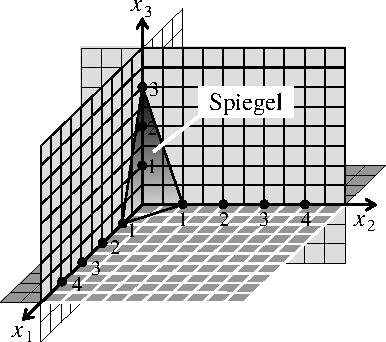
\includegraphics[width=.5\textwidth]{ma_007_spiegelmuseum.pdf}
		\caption{Skizze des Museumsraumes.}
		\label{fig:007_spiegel}
	\end{figure}
	
	\paragraph{a)} Stellen Sie eine Parametergleichung der Ebene $e$ auf, in der der Spiegel liegt. Entnehmen Sie die notwendigen Informationen aus der Abbildung.
	\begin{equation}
		e: \overrightarrow{x}=\left(\begin{array}{r} 0 \\ 0 \\ 3\end{array}\right) + \lambda \cdot \left(\begin{array}{r} 1 \\ 0 \\ -3\end{array}\right) + \mu \cdot \left(\begin{array}{r} 0 \\ 1 \\ -3\end{array}\right) \text{ mit } \lambda,\,\mu \in \mathbb{R} \text{ und } \lambda + \mu \leq 1
	\end{equation}
	
	\paragraph{b)} Zeigen Sie, dass der Punkt $S(\frac{1}{3}|\frac{1}{2}|\frac{1}{2})$ auf der Spiegelfläche liegt.
	\begin{equation}
		\left(\begin{array}{r} 0,\overline{3} \\ 0,5 \\ 0,5\end{array}\right) = \left(\begin{array}{r} 0 \\ 0 \\ 3\end{array}\right) + \lambda \cdot \left(\begin{array}{r} 1 \\ 0 \\ -3\end{array}\right) + \mu \cdot \left(\begin{array}{r} 0 \\ 1 \\ -3\end{array}\right)
	\end{equation}
	
	Um die Bedingung für die $x_1$-Koordinate zu erfüllen, muss intuitiv gelten:
	\begin{equation}
		x_1 = 0,\overrightarrow{3} = 0 + \lambda \cdot 1 + \mu \cdot 0 \Leftrightarrow \lambda = 0,\overline{3}.
	\end{equation}
	
	Um die Bedingung für die $x_2$-Koordinate zu erfüllen, muss intuitiv gelten:
	\begin{equation}
		x_2 = 0,5 = 0 + \lambda \cdot 0 + \mu \cdot 1 \Leftrightarrow \mu = 0,5.
	\end{equation}
	
	Einsetzen von $\lambda$ und $\mu$ gibt für die $x_3$-Koordinate:
	\begin{equation}
		x_3 = 3 + \frac{1}{3} \cdot (-3) + 0,5 \cdot (-3) = 0,5 \checkmark
	\end{equation}
	
	Die notwendige Bedingung $\lambda + \mu \leq 1$ ist ebenfalls erfüllt, denn
	\begin{equation}
		0,\overline{3} + 0,5 = 0,8\overline{3} \leq 1
	\end{equation}
	
	$\qed$
	
	\subsection{Ebenengleichungen}
	Geben Sie eine Gleichung der beschriebenen Ebene in Koordinatenform an.
	\paragraph{a)} $e_1$ ist eine Parallelebene zur $x_1$-$x_2$-Ebene durch den Punkt $P(1|2|3)$.
	\begin{equation}
		e_1: x_3 = 3 \Leftrightarrow x_3 - 3 = 0
	\end{equation}
	
	\paragraph{b)} $e_2$ ist eine Parallelebene zur $x_2$-$x_3$-Ebene durch den Punkt $Q(5|-2|-1)$.
	\begin{equation}
		e_2: x_1 = 5 \Leftrightarrow x_1 - 5 = 0
	\end{equation}
	
	\paragraph{a)} $e_3$ ist eine Parallelebene zur $x_1$-$x_3$-Ebene durch den Punkt $R(-1|-3|-2)$.
	\begin{equation}
		e_1: x_2 = -3 \Leftrightarrow x_2 +3 = 0
	\end{equation}
	
	\subsection{Noch mehr Ebenengleichungen}
	Geben Sie eine Koordinatengleichung der Ebenen an, die durch die markierten Flächen ausschnittsweise dargestellt sind.
	
	\begin{figure}[ht]
		\centering
		\begin{minipage}[b]{0.2\textwidth}
			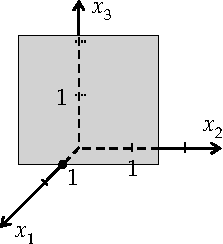
\includegraphics[width=\textwidth]{ma_008_flache1.pdf}
			\label{fig:008_flache1}
			\begin{center}
				a)
			\end{center}
		\end{minipage}
		\hfill
		\begin{minipage}[b]{0.2\textwidth}
			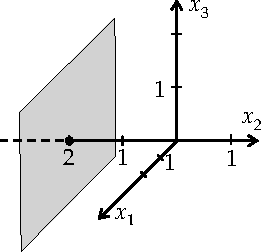
\includegraphics[width=\textwidth]{ma_009_flache2.pdf}
			\label{fig:009_flache2}
			\begin{center}
				b)
			\end{center}
		\end{minipage}
		\hfill
		\begin{minipage}[b]{0.2\textwidth}
			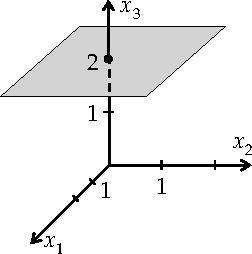
\includegraphics[width=\textwidth]{ma_010_flache3.pdf}
			\label{fig:010_flache3}
			\begin{center}
				c)
			\end{center}
		\end{minipage}
	\end{figure}
	
	\paragraph{a)} Fläche ist senkrecht zur $x_1$-Achse.
	\begin{equation}
		e_1: x_1 - 1 = 0
	\end{equation}
	
	\paragraph{b)} Fläche ist senkrecht zur $x_2$-Achse.
	\begin{equation}
		e_2: x_2 + 2 = 0
	\end{equation}
	
	\paragraph{c)} Fläche ist senkrecht zur $x_3$-Achse.
	\begin{equation}
		e_3: x_3 - 2 = 0
	\end{equation}
	
	\subsection{Achsenabschnittsform}
	Wandeln Sie die Gleichungen der Ebenen in die Achsenabschnittsform um.
	
	\paragraph{a)} $e_a: 2x_1 + x_2 + 2x_3 = 4$
	\begin{equation}
		e_a: \frac{x_1}{2} + \frac{x_2}{4} + \frac{x_3}{2} = 1
	\end{equation}
	
	\paragraph{b)} $e_b: 4x_1 - 3x_2 - 8x_3 = 12$
	\begin{equation}
		e_b: \frac{x_1}{3} - \frac{x_2}{4} - \frac{x_3}{\frac{2}{3}} = 1
	\end{equation}
	
	\paragraph{c)} $e_c: 3x_1 - 2x_3 = 6$
	\begin{equation}
		e_c: \frac{x_1}{2} - \frac{x_3}{3} = 1
	\end{equation}
	
	\paragraph{d)} $e_d: 3x_1 - 6 = 0$
	\begin{equation}
		e_d: \frac{x_1}{2} = 1
	\end{equation}
	
\end{document}